  \begin{minipage}[b]{0.45\linewidth}
  \centering
  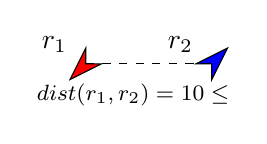
\begin{tikzpicture}[scale=0.8]
    \draw[fill=blue] (3,3) -- (2.75,3) -- (3.25,3.25) -- (3,2.75) -- cycle;
    \draw[fill=red] (1,3) -- (1,3.25) -- (0.75,2.75) -- (1.25,3)  -- cycle;
    \draw[dashed](1,3) -- (3,3);
    \node[] at (0.5, 3.3) {$r_1$};
    \node[] at (2.5, 3.3) {$r_2$};
    \node[] at (1.75, 2.5) {\footnotesize{$\operatorname{dist}(r_1, r_2)=10 \leq \range$}};
  \end{tikzpicture}
  \end{minipage}
\begin{minipage}[b]{0.45\linewidth}
  \centering
  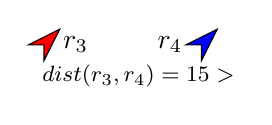
\begin{tikzpicture}[scale=0.8]
    \draw[fill=blue] (3.5,3) -- (3.25,3) -- (3.75,3.25) -- (3.5,2.75) -- cycle;
    \draw[fill=red] (1,3) -- (0.75,3) -- (1.25,3.25) -- (1,2.75) -- cycle;
    \node[] at (1.5, 3) {$r_3$};
    \node[] at (3, 3) {$r_4$};
    \node[] at (2.5, 2.5) {\footnotesize{$\operatorname{dist}(r_3, r_4)=15 > \range$}};
  \end{tikzpicture}
\end{minipage}
\caption{Consider a special instance of lattice graph in
  Figure~\ref{fig:edgetrans}, assume the range $\range = 10$, edge length $l=10$,
  $\alpha=3\pi/4, \beta=\pi/4$. [left] Two robots $r_1, r_2$ satisfy the lattice
  graph with $\Q=1$. [right] Two robots $r_3, r_4$ can not observe each other, but
  they satisfy the lattice graph with $\Q=0$.}
